%%%%%%%%%%%%
%
% $Autor: Leon Ritscher $
% $Datum: 2025-06-01 $

% !TeX spellcheck = en_GB/de_DE
% !TeX encoding = utf8
% !TeX root = filename 
% !TeX TXS-program:bibliography = txs:///biber
%
%%%%%%%%%%%%

% Structure
\chapter{Wippschalter}
\label{ch:Wippschalter}

\section{Allgemeine Beschreibung}

Wippschalter sind elektromechanische Aktoren, welche der manuellen Umschaltung eines elektrischen Signals dienen, wie z.B. das Ein- und Ausschalten eines Geräts. Sie besitzen typischerweise zwei oder mehr stabile Schaltstellungen und arbeiten als rastende Schalter mit mechanischer Verriegelung. In Mikrocontroller-Anwendungen können Wippschalter verwendet werden, um zwischen verschiedenen Betriebsmodi zu wechseln oder bestimmte Funktionen zu aktivieren/deaktivieren.

\section{Zweipoliger Wippschalter}

Ein zweipoliger Wippschalter \ref{fig:Wippschalter} besitzt zwei Eingangskontakte L1 und L2 und zwei korrespondierende Ausgangskontakte T1 und T2. Diese werden gleichzeitig geöffnet oder geschlossen \cite{reichelt_wippschalter_1552_2021}. Das Design ermöglicht eine einfache Bedienung durch Kippen der Wippe, um zwischen den beiden Schaltzuständen zu wechseln.

\begin{figure}
	\centering
	\resizebox{0.6\textwidth}{!}{%
		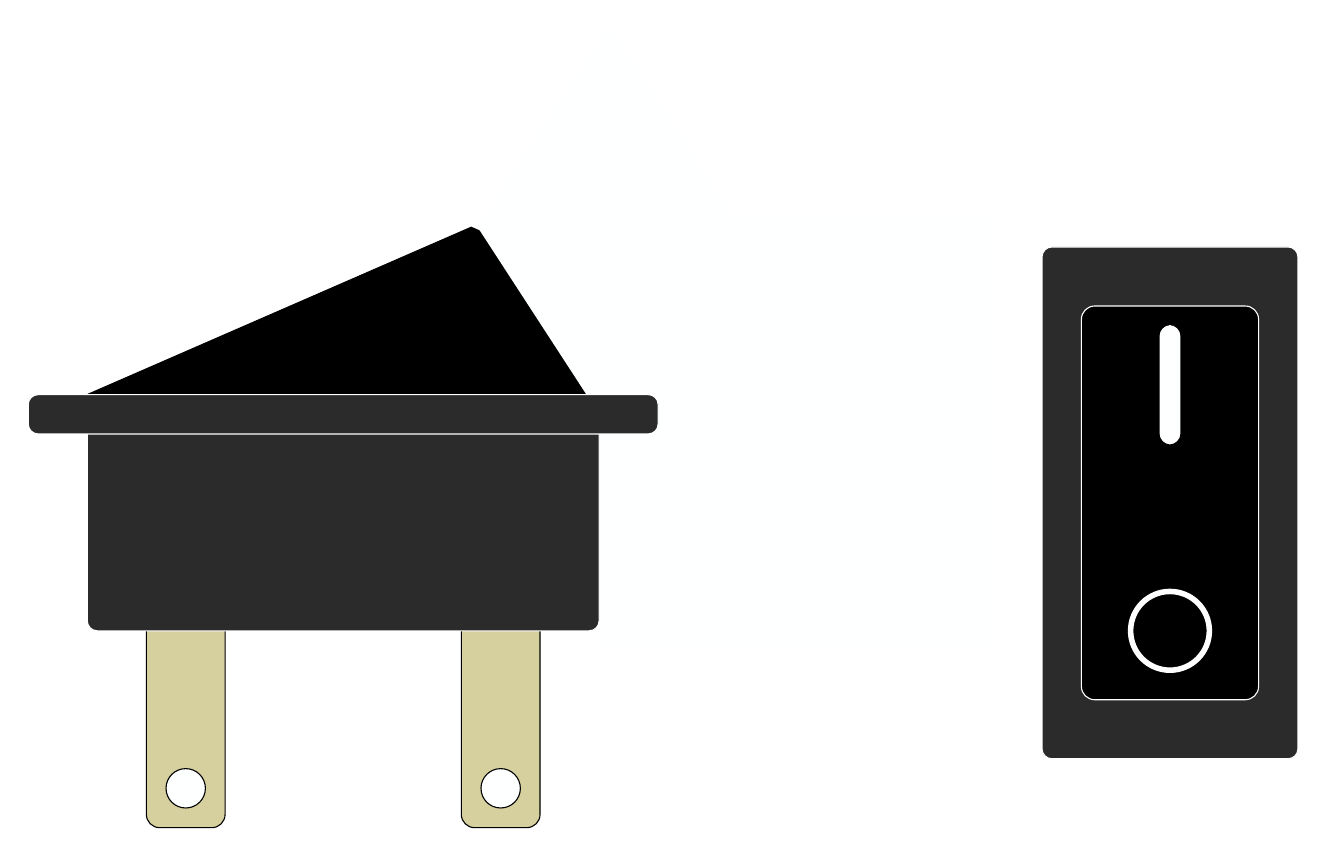
\begin{tikzpicture}
			\tikzstyle{every node}=[font=\Huge]
			\draw [ fill={rgb,255:red,214; green,207; blue,158} , rounded corners = 4.8] (14,16) rectangle (15,13.25);
			\draw [ fill={rgb,255:red,214; green,207; blue,158} , rounded corners = 4.8] (10,16) rectangle (11,13.25);
			\draw [ fill={rgb,255:red,0; green,0; blue,0} ] (9.25,18.75) -- (14.125,20.875) -- (19,18.75) -- (14.125,16.625) -- cycle;
			\draw [ color={rgb,255:red,254; green,255; blue,255} , fill={rgb,255:red,254; green,255; blue,255}] (15.75,21) rectangle  node {\LARGE Text} (20.75,15.5);
			\draw [ color={rgb,255:red,255; green,255; blue,255} , fill={rgb,255:red,43; green,43; blue,43}, rounded corners = 3.6] (15.75,15.75) rectangle (9.25,18.5);
			\draw [ color={rgb,255:red,254; green,255; blue,255} , fill={rgb,255:red,254; green,255; blue,255}, line width=2pt ] (14.25,20.875) -- (15.875,18.375) -- (17.5,20.875) -- (15.875,23.375) -- cycle;
			\draw [ color={rgb,255:red,255; green,255; blue,255} , fill={rgb,255:red,43; green,43; blue,43}, rounded corners = 3.6] (8.5,18.75) rectangle (16.5,18.25);
			\draw [ fill={rgb,255:red,254; green,255; blue,255} ] (10.5,13.75) circle (0.25cm);
			\node [font=\LARGE, color={rgb,255:red,255; green,255; blue,255}] at (14.25,14.5) {};
			\draw [ fill={rgb,255:red,254; green,255; blue,255} ] (14.5,13.75) circle (0.25cm);
			\draw [ color={rgb,255:red,255; green,255; blue,255} , fill={rgb,255:red,43; green,43; blue,43}, rounded corners = 3.6, rotate around={-90:(23, 17.375)}] (26.25,15.75) rectangle (19.75,19);
			\draw [ color={rgb,255:red,255; green,255; blue,255} , fill={rgb,255:red,0; green,0; blue,0}, rounded corners = 4.8, rotate around={-90:(23, 17.375)}] (20.5,18.5) rectangle (25.5,16.25);
			\draw [ color={rgb,255:red,255; green,255; blue,255} , fill={rgb,255:red,254; green,255; blue,255}, rounded corners = 3.8, rotate around={-90:(23, 18.875)}] (22.25,19) rectangle (23.75,18.75);
			\draw [ color={rgb,255:red,255; green,255; blue,255} , fill={rgb,255:red,0; green,0; blue,0}, line width=2pt ] (23,15.75) ellipse (0.5cm and 0.5cm);
		\end{tikzpicture}
	}%
	\caption{Seiten- und Draufsicht des Wippschalters}
	\label{fig:Wippschalter}
\end{figure}

\section{Eigenschaften}

Aus dem Datenblatt \cite{reichelt_wippschalter_1552_2021} lassen sich folgende Eigenschaften des Moduls entnehmen:

\begin{itemize}
	\item Schaltfunktion: zweipolig, rastend (DPST, EIN/AUS)
	\item Bemessungsspannung: 250\,V AC
	\item Bemessungsstrom: bis 16\,A (ohmsche Last)
	\item Einschaltspitzenstrom: maximal 100\,A (kapazitive Last, kurzzeitig)
	\item Kontaktwiderstand: $< 100\,\mathrm{m\Omega}$ bei 1\,A, 12\,V DC
	\item Isolationswiderstand: $> 100\,\mathrm{M\Omega}$ bei 500\,V DC
	\item Kontaktabstand: $\geq 3\,\mathrm{mm}$ (nach VDE)
	\item Kriechstromfestigkeit: 250\,PTI (Proof Tracking Index)
	\item Mechanische Lebensdauer: $\geq 50{,}000$ Schaltspiele
	\item Betriebstemperatur (Anschlussseite): $-20\,^{\circ}\mathrm{C}$ bis $+100\,^{\circ}\mathrm{C}$
	\item Betriebstemperatur (Betätigungsseite): $-20\,^{\circ}\mathrm{C}$ bis $+55\,^{\circ}\mathrm{C}$
	\item Glühdrahttesttemperatur: 850\,°C (nach IEC 60695-2-11)
	\item Gehäuse- und Betätigermaterial: PA (Polyamid), UL 94 V-2, flammhemmend
	\item Schutzklasse: geeignet für Geräte der Schutzklasse II
	\item Anschlussart: Flachsteckanschlüsse 6{,}3\,×\,0{,}8\,mm
	\item Einbauart: Snap-in (Frontplattenmontage)
	\item Gerätewanddicke: 0{,}8\,mm bis 5{,}0\,mm
	\item Aufsteckkraft (Steckhülsen): ca. 80\,N
	\item Einbaumaß: ca. 27{,}2\,×\,12{,}2\,mm
\end{itemize}